\chapter{Introduction}\label{ch:intro} % 1

Parallel programming---that is, writing programs that can take
advantage of parallel hardware to go faster---is notoriously
difficult.  A fundamental reason for this difficulty is that programs
can yield inconsistent results, or even crash, due to unpredictable
interactions between parallel tasks.

\emph{Deterministic-by-construction} parallel programming models,
though, offer the promise of freedom from subtle, hard-to-reproduce
nondeterministic bugs in parallel code. Although there are many ways to
construct individual deterministic programs and verify their
determinism, deterministic-by-construction programming models provide
a \emph{language-level} guarantee of determinism
that holds for all programs written using the model.

A deterministic program is one that has the same \emph{observable
  behavior} every time it is run.  How do we define what is observable
about a program's behavior?  Certainly, we do \emph{not} wish to
preserve behaviors such as running time across multiple
runs---ideally, a deterministic parallel program will run faster when
more parallel resources are available.  Moreover, we do not want to
count scheduling behavior as observable---in fact, we want to
specifically \emph{allow} tasks to be scheduled dynamically and
unpredictably, without allowing such \emph{schedule nondeterminism} to
affect the observable behavior of a program.  Therefore, \either{in this
dissertation I will define}{we will define} the observable behavior of a program to be
\emph{the value to which the program evaluates}.

\lk{In my proposal, I had a footnote here: ``We assume that programs
  have no side effects other than state effects.'' I think I instead
  just want to say that we \emph{ignore} other side effects.  They can
  \emph{happen}; it's just that they don't count.}

This definition of observable behavior ignores side effects other than
\emph{state}.  But even with such a limited notion of what is
observable, schedule nondeterminism can affect the outcome of a
program.  For instance, if a computation writes $3$ to a shared
location while another computation writes $4$, then a subsequent third
computation that reads and returns the location's contents will
nondeterministically return $3$ or $4$, depending on the order in
which the first two computations ran.  Therefore, if a parallel
programming model is to guarantee determinism by construction, it must
necessarily limit sharing of mutable state between parallel tasks in
some way.

\section{The deterministic-by-construction parallel programming landscape}\label{s:intro-landscape}

There is long-standing work on deterministic-by-construction parallel
programming models that limit sharing of state between tasks. The
possibilities include:

\begin{itemize}
\item \emph{No-shared-state parallelism.}  One classic approach to
  guaranteeing determinism in a parallel programming model is to allow
  \emph{no} shared mutable state between tasks, forcing tasks to
  produce values independently.  An example of no-shared-state
  parallelism is pure functional programming with function-level task
  parallelism, or \emph{futures}---for instance, in Haskell programs
  that use the @par@ and @pseq@ combinators~\cite{marlow-par}.  The
  key characteristic of this style of programming is lack of side
  effects: because programs do not have side effects, expressions can
  evaluate simultaneously without affecting the eventual value of the
  program.  Also belonging in this category are parallel programming
  models based on \emph{pure data parallelism}, such as Data Parallel
  Haskell~\cite{dph, dph-status} or the River Trail API for
  JavaScript~\cite{river-trail}, each of which extend existing
  languages with \emph{parallel array} data types and (observably)
  pure operations on them.

\item \emph{Data-flow parallelism.}  In \emph{Kahn process networks}
  (KPNs)~\cite{Kahn-1974}, as well as in the more restricted
  \emph{synchronous data flow} systems~\cite{Lee-sdn}, a network of
  independent ``computing stations'' communicate with each other
  through first-in, first-out (FIFO) queues, or \emph{channels}.  In
  this model, each computing station is a task, and channels are the
  only means of sharing state between tasks.  Furthermore, reading
  data from a channel is a \emph{blocking} operation: once an
  attempt to read has started, a computing station cannot do anything
  else until the data to be read is available.  Each station computes
  a sequential, monotonic function from the \emph{history} of its
  input channels (\ie, the input it has received so far) to the
  history of its output channels (the output it has produced so far).
  KPNs are the basis for deterministic stream-processing languages
  such as StreamIt~\cite{streamit-asplos}.

\item \emph{Single-assignment parallelism.}  In parallel
  \emph{single-assignment} languages, ``full/empty'' bits are
  associated with memory locations so that they may be written to at
  most once. Single-assignment locations with blocking read semantics
  are known as \emph{IVars}~\cite{IStructures} and are a
  well-established mechanism for enforcing determinism in parallel
  settings: they have appeared in Concurrent ML as
  @SyncVar@s~\cite{reppy-cml-book}; in the Intel Concurrent
  Collections (abbreviated ``CnC'') system~\cite{CnC}; and have even
  been implemented in hardware in Cray MTA machines~\cite{cray-mta}.
  Although most of these uses of IVars incorporate them into
  already-nondeterministic programming environments, the
  \emph{monad-par} Haskell library~\cite{monad-par} uses IVars in a
  deterministic-by-construction setting, allowing user-created threads
  to communicate through IVars without requiring the @IO@ monad.
  Rather, operations that read and write IVars must run inside a @Par@
  monad, thus encapsulating them inside otherwise pure programs, and
  hence a program in which the only effects are @Par@ effects is
  guaranteed to be deterministic.

\item \emph{Imperative disjoint parallelism.}  Finally, yet another
  approach to guaranteeing determinism is to ensure that the state
  accessed by concurrent threads is \emph{disjoint}.  Sophisticated
  permissions systems and type systems can make it possible for imperative
  programs to mutate state in parallel, while guaranteeing that the
  same state is not accessed simultaneously by multiple threads.  \either{I}{We}
  will refer to this style of programming as \emph{imperative disjoint
    parallelism}, with Deterministic Parallel Java
  (DPJ)~\cite{dpj-oopsla, dpj-hotpar09} as a prominent example.
\end{itemize}

\ifdefined\DISSERTATION
\begin{wrapfigure}{r}{3in}
\vspace{-2em}
\begin{center}
  
\includegraphics[scale=0.18]{../illustrations/sharing-state}
\end{center}
\vspace{-1.5em}
\end{wrapfigure}
\fi
The four parallel programming models listed above---no-shared-state
parallelism, data-flow parallelism, single-assignment parallelism, and
imperative disjoint parallelism---all seem to embody rather different
mechanisms for exposing parallelism and for ensuring determinism.  If
we view these different programming models as a toolkit of unrelated
choices, though, it is not clear how to proceed when we want to
implement an application with multiple parallelizable components that
are best suited to different programming models.  For example, suppose
we have an application in which we want to exploit data-flow pipeline
parallelism via FIFO queues, but we also want to mutate disjoint slices of
arrays.  It is not obvious how to compose two programming models that
each only allow communication through a single type of shared data
structure---and if we do manage to compose them, it is not obvious whether the
determinism guarantee of the individual models is preserved by their
composition.  Therefore, we seek a general, broadly-applicable model
for deterministic parallel programming that is not tied to a
particular data structure.

\section{Monotonic data structures as a basis for deterministic parallelism}\label{s:intro-monotonic}

In KPNs and other data-flow models, communication takes place over
blocking FIFO queues with ever-increasing \emph{channel histories},
while in IVar-based programming models such as CnC and monad-par, a
shared data store of blocking single-assignment memory locations grows
monotonically.  Hence \emph{monotonic data structures}---data
structures to which information can only be added and never removed,
and for which the timing of updates is not observable---emerge as a
common theme of guaranteed-deterministic programming models.

In this \either{dissertation, I}{paper, we} show that \emph{lattice-based} data
structures, or \emph{LVars}, offer a general approach to deterministic
parallel programming that takes monotonicity as a starting point. The
states an LVar can take on are elements of a given
\emph{lattice}.  This lattice determines the
semantics of the @put@ and @get@ operations that comprise the
interface to LVars (which \either{I}{we} will explain in detail in
\either{Chapter}{Section}~\ref{ch:lvars}):
\begin{itemize}
\item The @put@ operation can only make the state of an LVar ``grow''
  with respect to the lattice, because it updates the LVar to the
  \emph{least upper bound} of the current state and the new state.
  For example, on LVars of collection type, such as sets, the @put@ operation
  typically inserts an element.

\item The @get@ operation allows only limited observations of the
  contents of an LVar.  It requires the user to specify a
  \emph{threshold set} of minimum values that can be read from the
  LVar, where every two elements in the threshold set must have the
  lattice's greatest element $\top$ as their least upper bound.  A
  call to @get@ blocks until the LVar in question reaches a (unique)
  value in the threshold set, then unblocks and returns that value.
\end{itemize}
Together, least-upper-bound writes via @put@ and threshold reads via
@get@ yield a programming model that is deterministic by construction.  That
is, a program in which @put@ and @get@ operations on LVars are the
only side effects will have the same observable result every time it is run, regardless of
parallel execution and schedule nondeterminism.  As we will see in \either{Chapter}{Section}~\ref{ch:lvars}, no-shared-state parallelism, data-flow
parallelism and single-assignment parallelism are all subsumed by the
LVars programming model, and as we will see in
Section~\ref{s:lvish-disjoint}, imperative disjoint parallel updates
are compatible with LVars as well.

Furthermore, as \either{I}{we} show in
Section~\ref{s:lvars-generalizing}, 
\ifdefined\DISSERTATION
we can generalize the behavior of
the @put@ and @get@ operations while retaining determinism: we can
generalize from the least-upper-bound @put@ operation to a set of
arbitrary \emph{update operations} that are not necessarily idempotent
(but are still inflationary and commutative), and we can generalize
the @get@ operation to allow a more general form of threshold reads.
Generalizing from @put@ to arbitrary inflationary and commutative
updates turns out to be a particularly useful extension to the LVars
model; \either{I}{we} formally extend the model to support these update operations
in \either{Chapter}{Section}~\ref{ch:quasi}, and in \either{Chapter}{Section}~\ref{ch:lvish} \either{I}{we} discuss how
arbitrary update operations are useful in practice.
\fi
\ifdefined\JOURNAL
we can generalize from the least-upper-bound @put@ operation to a set
of arbitrary \emph{update operations} that are not necessarily
idempotent (but are still inflationary and commutative), while
retaining determinism.  This generalization turns out to be a
particularly useful extension to the LVars model; \either{I}{we}
formally extend the model to support these arbitrary update operations
in \either{Chapter}{Section}~\ref{ch:quasi}, and in
\either{Chapter}{Section}~\ref{ch:lvish} \either{I}{we} discuss how
arbitrary update operations are useful in practice.
\fi

\section{Quasi-deterministic and event-driven programming with LVars}\label{s:intro-quasi}

The LVars model described above guarantees determinism and supports an
unlimited variety of shared data structures: anything viewable as a
lattice.  However, it is not as general-purpose as one might hope.
Consider, for instance, an algorithm for unordered graph traversal.  A
typical implementation involves a monotonically growing set of ``seen
nodes''; neighbors of seen nodes are fed back into the set until it
reaches a fixed point.  Such fixpoint computations are ubiquitous, and
would seem to be a perfect match for the LVars model due to their use
of monotonicity.  But they are not expressible using the threshold
@get@ and least-upper-bound @put@ operations, nor even with the more
general \either{alternatives to \lstinline|get| and \lstinline|put|}{update operations} mentioned above.

The problem is that these computations rely on \emph{negative}
information about a monotonic data structure, \ie, on the
\emph{absence} of certain writes to the data structure.  In a graph
traversal, for example, neighboring nodes should only be explored if
the current node is \emph{not yet} in the set; a fixpoint is reached
only if no new neighbors are found; and, of course, at the end of the
computation it must be possible to learn exactly which nodes were
reachable (which entails learning that certain nodes were not).  In \either{Chapter}{Section}~\ref{ch:quasi}, \either{I}{we} describe two extensions to the basic LVars
model that make such computations possible:
\begin{itemize}
\item First, \either{I}{we} add the ability to attach \emph{event handlers} to an
  LVar.  When an event handler has been registered with an LVar, it
  causes a callback function to run, asynchronously, whenever
  events arrive (in the form of monotonic updates to the LVar).
  Crucially, it is possible to check for \emph{quiescence} of a group
  of handlers, discovering that no callbacks are currently enabled---a
  transient, negative property.  Since quiescence means that there are
  no further changes to respond to, it can be used to tell that a
  fixpoint has been reached.
\item Second, \either{I}{we} extend the model with a primitive operation @freeze@
  for \emph{freezing} an LVar, which allows its contents to be read
  immediately and exactly, rather than the blocking threshold read
  that @get@ allows.  The @freeze@ primitive imposes the following
  trade-off: once an LVar has been frozen, any further writes that
  would change its value instead raise an exception; on the other
  hand, it becomes possible to discover the exact value of the LVar,
  learning both positive and negative information about it, without
  blocking.  Therefore, LVar programs that use @freeze@ are \emph{not}
  guaranteed to be deterministic, because they could
  nondeterministically raise an exception depending on how writes and
  @freeze@ operations are scheduled.  However, such programs satisfy
  \emph{quasi-determinism}: all executions that produce a final value
  (instead of raising an exception)
  produce the \emph{same} final value.
\end{itemize}

Writes to an LVar could cause more events to occur after a group of handlers associated
with that LVar has quiesced, and those events could trigger more
invocations of callback functions.  However, since the contents of the
LVar can only be read through @get@ or @freeze@
operations anyway, early quiescence poses no risk to determinism or
quasi-determinism, respectively.  In fact, freezing and quiescence
work particularly well together because freezing provides a mechanism
by which the programmer can safely ``place a bet'' that all writes to an LVar
have completed.  Hence freezing and handlers make it possible to implement fixpoint
computations like the graph traversal described above.  Moreover, if
we can ensure that a freeze does indeed happen after all writes to the LVar in question have
completed, then we can ensure that the entire computation is deterministic,
and it is possible to enforce this ``freeze-last'' idiom at the
implementation level, as \either{I}{we} discuss below (and, in more detail, in
Section~\ref{subsection:lvish-regaining-full-determinism-with-runparthenfreeze}).

\section{The LVish library}\label{s:intro-lvish}

To demonstrate the practicality of the LVars programming model, \either{in
Chapter~\ref{ch:lvish} I will describe}{we have implemented}
\emph{LVish}, a Haskell library\footnote{Available at
  \url{http://hackage.haskell.org/package/lvish}.}
for deterministic and quasi-deterministic programming with LVars.

LVish provides a @Par@ monad for encapsulating parallel computations.\footnote{The
  \lstinline|Par| monad exposed by LVish generalizes the original
  \lstinline|Par| monad exposed by the \emph{monad-par} library
  ({\url{http://hackage.haskell.org/package/monad-par}}, described by
  Marlow \etal~\cite{monad-par}), which allows determinism-preserving
  communication between threads, but only through IVars, rather than
  LVars.}
A @Par@ computation can create lightweight, library-level threads that
are dynamically scheduled by a custom work-stealing scheduler.
LVar operations run inside the @Par@ monad, which is
indexed by an \emph{effect level}, allowing fine-grained specification
of the effects that a given computation is allowed to perform.  For
instance, since @freeze@ introduces quasi-determinism, a computation
indexed with a deterministic effect level is not allowed to use
@freeze@.  Thus, the \emph{type} of an LVish computation reflects its
determinism or quasi-determinism guarantee.  Furthermore, if a
@freeze@ is guaranteed to be the \emph{last} effect that occurs in a
computation, then it is impossible for that @freeze@ to race with a
write, ruling out the possibility of a run-time write-after-freeze
exception.  LVish exposes a @runParThenFreeze@ operation that captures
this ``freeze-last'' idiom and has a deterministic effect level.

LVish also provides a variety of lattice-based data structures (\eg,
sets, maps, arrays) that support concurrent insertion, but not
deletion, during @Par@ computations.  Users may also implement their own lattice-based data structures,
and LVish provides tools to facilitate the definition of user-defined
LVars.  \either{I will describe}{In Section~\ref{ch:lvish}, we describe} the proof obligations for LVar
implementors and give examples of applications that use user-defined
LVars as well as those that the library provides.

Finally, \either{Chapter}{Section}~\ref{ch:lvish}
illustrates LVish through two case studies, drawn from \either{my
collaborators' and my}{our} experience using the LVish library, both of which
make use of handlers and freezing:
\begin{itemize}
\item First, \either{I}{we} describe using LVish to parallelize a control flow
  analysis ($k$-CFA) algorithm.  The goal of $k$-CFA is to compute the
  flow of values to expressions in a program.  The $k$-CFA algorithm
  proceeds in two phases: first, it explores a graph of \emph{abstract
    states} of the program; then, it summarizes the results of the
  first phase.  Using LVish, these two phases can be pipelined;
  moreover, the original graph exploration phase can be internally
  parallelized.  \either{I}{We} contrast our LVish implementation with the original
  sequential implementation from which it was ported and give performance results.
\item Second, \either{I}{we} describe using LVish to parallelize
  \emph{PhyBin}~\cite{PhyBin}, a bioinformatics application for
  comparing sets of phylogenetic trees that relies heavily on a
  parallel tree-edit distance algorithm~\cite{hashrf}.  The PhyBin
  application crucially relies on the aforementioned ability to
  perform arbitrary inflationary and commutative (but not idempotent)
  updates on LVars (in contrast to the idempotent @put@ operation).
  We show that the performance of the parallelized PhyBin application
  compares favorably to existing widely-used software packages for
  analyzing collections of phylogenetic trees.
\end{itemize}

\ifdefined\DISSERTATION
\section{Deterministic threshold queries of distributed data structures}\label{s:intro-cvrdts}

The LVars model is closely related to the concept of
\emph{conflict-free replicated data types} (CRDTs)~\cite{crdts} for
enforcing \emph{eventual consistency}~\cite{vogels-ec} of replicated
objects in a distributed system.  In particular, \emph{state-based} or
\emph{convergent} replicated data types, abbreviated as
\emph{CvRDTs}~\cite{crdts, crdts-tr}, leverage the mathematical
properties of lattices to guarantee that all replicas of an object
(for instance, in a distributed database) eventually agree.

Although CvRDTs are provably eventually consistent, queries of CvRDTs
(unlike threshold reads of LVars) nevertheless allow inconsistent
intermediate states of replicas to be observed.  That is, if two
replicas of a CvRDT object are updated independently, reads of those
replicas may disagree until a (least-upper-bound) \emph{merge}
operation takes place.

Taking inspiration from LVar-style threshold reads, in
\either{Chapter}{Section}~\ref{ch:distributed} I show how to extend CvRDTs to support
deterministic, \emph{strongly consistent} queries using a mechanism
called \emph{threshold queries} (or, seen from another angle, I show
how to port threshold reads from a shared-memory setting to a
distributed one).  The threshold query technique generalizes to any
lattice, and hence any CvRDT, and allows deterministic observations to
be made of replicated objects before the replicas' states have
converged.  This work has practical relevance since, while real
distributed database applications call for a combination of eventually
consistent and strongly consistent queries, CvRDTs only support the
former.  Threshold queries extend the CvRDT model to support both
kinds of queries within a single, lattice-based reasoning framework.
Furthermore, since threshold queries behave deterministically
regardless of whether all replicas agree, they suggest a way to save
on synchronization costs: existing operations that require all
replicas
\begin{wrapfigure}{r}{1.4in}
  \vspace{-2em}
  \begin{center}
    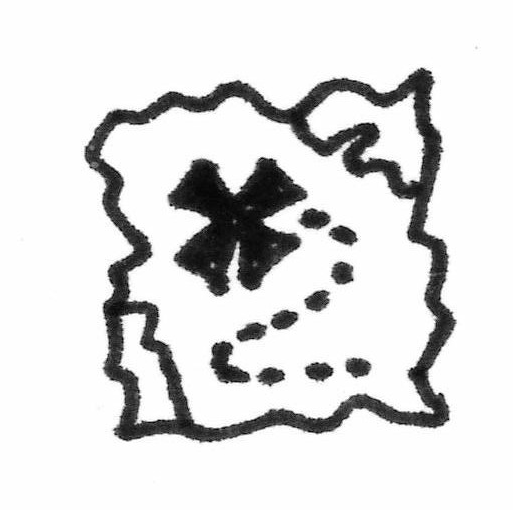
\includegraphics[scale=0.18]{../illustrations/map}
  \end{center}
  \vspace{-3em}
\end{wrapfigure}
to agree could be done with threshold queries instead, and
retain behavior that is \emph{observably} strongly consistent while
avoiding unnecessary synchronization.
\fi

\ifdefined\DISSERTATION
\section{Thesis statement, and organization of the rest of this dissertation}\label{s:intro-thesis}

With the above background, I can state my thesis:\lk{This format
  ripped off from Josh Dunfield.}
\begin{quote}
  Lattice-based data structures are a general and practical unifying
  abstraction for deterministic and quasi-deterministic parallel and
  distributed programming.
\end{quote}
\lk{Changed from ``foundation'' to ``unifying abstraction'' --
  otherwise it's the same as in my proposal.}  The rest of this
dissertation supports my thesis as follows:
\begin{itemize}
  \item \emph{Lattice-based data structures}: In
    Chapter~\ref{ch:lvars}, I formally define LVars and use them to
    define $\lambdaLVar$, a call-by-value parallel calculus with a
    store of LVars that support least-upper-bound @put@ and threshold
    @get@ operations. In Chapter~\ref{ch:quasi}, I extend
    $\lambdaLVar$ to add support for arbitrary update operations,
    event handlers, and the @freeze@ operation, calling the resulting
    language $\lambdaLVish$.  Appendix~\ref{app:plt-redex} contains
    runnable versions of $\lambdaLVar$ and $\lambdaLVish$ implemented
    using the PLT Redex semantics engineering system~\cite{redex-book}
    for interactive experimentation.

  \item \emph{general}: In Chapter~\ref{ch:lvars}, I show how
    previously existing deterministic parallel programming models
    (single-assignment languages, Kahn process networks) are subsumed
    by the lattice-generic LVars model.  Additionally, I show how to
    generalize the @put@ and @get@ operations on LVars while
    preserving their determinism.

  \item \emph{deterministic}: In Chapter~\ref{ch:lvars}, I show that
    the basic LVars model guarantees determinism by giving a proof of
    determinism for the $\lambdaLVar$ language with @put@ and @get@.

  \item \emph{quasi-deterministic}: In Chapter~\ref{ch:quasi}, I
    define quasi-determinism and give a proof of quasi-determinism for
    $\lambdaLVish$, which adds arbitrary update operations, the
    @freeze@ operation, and event handlers to the $\lambdaLVar$
    language of Chapter~\ref{ch:lvars}.

  \item \emph{practical} and \emph{parallel}: In
    Chapter~\ref{ch:lvish}, I describe the interface and
    implementation of the LVish Haskell library, which is based on the
    LVars programming model, and demonstrate how it is used for
    practical programming with the two case studies described above,
    including performance results on parallel hardware.\lk{I threw in
      ``parallel'' here because I wasn't counting it under any of the
      other bullets.  Parallelism is a resource; we have a ``parallel
      language semantics'' in the sense that it's a semantics that
      gives the scheduler lots of purchase to schedule it onto
      parallel hardware, and the only proof of that is in the pudding.
      So I'm not sure where else to support the claim of parallelism
      but here.}

  \item \emph{distributed programming}: In
    Chapter~\ref{ch:distributed}, I show how LVar-style threshold
    reads apply to the setting of distributed, replicated data
    structures.  In particular, I extend convergent replicated data
    types (CvRDTs) to support strongly consistent threshold queries,
    which take advantage of the existing lattice structure of CvRDTs
    and allow deterministic observations to be made of their contents
    without requiring all replicas to agree.
\end{itemize}
\fi

\section{Previously published work}

\ifdefined\DISSERTATION
The material in this dissertation is based in large part on research
done jointly with several collaborators, some of which appears in the
following previously published papers:

\lk{These are formatted in ``ACM Ref'' style.}

\begin{itemize}
\item Lindsey Kuper and Ryan
  R. Newton. 2013. \href{http://doi.acm.org/10.1145/2502323.2502326}{LVars:
    lattice-based data structures for deterministic parallelism.} In
  \emph{Proceedings of the 2nd ACM SIGPLAN Workshop on Functional
    High-Performance Computing} (FHPC '13).

\item Lindsey Kuper, Aaron Turon, Neelakantan R. Krishnaswami, and
  Ryan
  R. Newton. 2014. \href{http://doi.acm.org/10.1145/2535838.2535842
  }{Freeze after writing: quasi-deterministic parallel programming
    with LVars.} In \emph{Proceedings of the 41st ACM SIGPLAN-SIGACT
    Symposium on Principles of Programming Languages} (POPL '14).

\item Lindsey Kuper and Ryan
  R. Newton. 2014. \href{http://wodet.cs.washington.edu/wp-content/uploads/2014/02/wodet2014-final1.pdf}{Joining
    forces: toward a unified account of LVars and convergent
    replicated data types.} In the \emph{5th Workshop on Determinism
    and Correctness in Parallel Programming} (WoDet '14).

\item Lindsey Kuper, Aaron Todd, Sam Tobin-Hochstadt, and Ryan
  R. Newton. 2014. \href{http://doi.acm.org/10.1145/2594291.2594312
  }{Taming the parallel effect zoo: extensible deterministic
    parallelism with LVish.} In \emph{Proceedings of the 35th ACM
    SIGPLAN Conference on Programming Language Design and
    Implementation} (PLDI '14).
\end{itemize}

\lk{I was going to put something like, ``The material in this chapter
  is based on research done jointly with...'' in individual chapters,
  and cite each paper at the start of its chapter.  But chapters don't
  really correspond to the papers, so I'm just going to try citing all
  the papers up front like this.  In particular, Chapter 2 is a hybrid
  of the first and second papers listed above, except for material in
  Section 2.6, which is new; Chapter 3 is based on the second paper
  listed above; except for everything pertaining to update operations,
  which is new; Chapter 4 is based on the second and fourth papers
  listed above; and Chapter 5 is based very loosely on the third paper
  listed above, but is largely new (and we have an as-yet-unpublished
  new paper about it).  If this is actually useful information, I'll
  add it; if not, I'll leave it out.}
\fi

\ifdefined\JOURNAL

This paper revises and expands on our previously published work on
LVars and LVish~\cite{Freeze-paper, LVars-paper, effectzoo}.
The $\lambdaLVar$ calculus of Section~\ref{ch:lvars}
is a hybrid of the LVars formalisms presented in our previous papers,
and the $\lambdaLVish$ calculus of Section~\ref{ch:quasi} is based on
the previously-published \emph{LVish calculus}~\cite{Freeze-paper},
but generalizes it to allow the arbitrary update operations  described
above and in Section~\ref{s:lvars-generalizing}.  Additionally, Section~\ref{ch:lvish} describes the current version of the LVish Haskell library, which has been updated to run
against the current version\footnote{GHC 7.8.3, at the time of
  this writing.} of the Glasgow Haskell Compiler, and all the code
examples in the paper run against this newest version of LVish.

\fi
